\chapter{Recurrent Neural Network} \label{ch:rnn}

\section{Brief Review of RNN}

RNN is a connectionist model with the ability to selectively pass information across sequence steps \cite{lipton2015critical}. It is good at handling sequence of data such as voice message, text contents, or a flow of images (videos). It is worth mentioning that the ``sequence'' does not necessarily mean a time sequence. Nevertheless, without losing generality, we will consider time sequence in the review for simplicity and convenience.

Denote inputs $x(1), x(2), ..., x(k), ...$ where $x(k)$ is a vector sampled at time instant $k$. The length of the sequence may be finite or infinite. In the case of finite sequence, its maximum sample index is denoted by $T$. For example, in the context of natural language processing, each input might be a word in a dictionary. For example, $x(1) = \textup{``Pandas''}$, $x(2)=\textup{``are''}$, $x(3)=\textup{``so''}$, $x(4)=\textup{``cute''}$, $x(5)=\textup{``!''}$. The corresponding target output sequence is given by $y(1), y(2), ..., y(k), ...$, respectively.

RNN differs from the conventional dense ANN by introducing ``recurrent edges'', which allows the output of hidden layers at $k-1$ be used as additional inputs to the system at $k$. This means, at any time $k$, the input of the system includes both $x(k)$ and also selected $h(k-1)$, where $h(\cdot)$ is the outputs of hidden layers. We can think of the ``weights'' of a trained RNN the ``long-term memory'' that does not change with specific sequence of inputs, while the information passing through recurrent edges the ``short-term memory'' that links previous inputs with future inputs.

A demonstration is given in Fig. \ref{ch:rnn:fig:rnn_general}. Notice that each hidden layer is a multi-input-multi-output subsystem containing multiple nodes. Different from a conventional dense ANN, each hidden layer takes additional inputs from its corresponding hidden layer in the previous instant. It is also common to see ``bypass'' (this is widely used in different ANN structures, not unique to RNN) for better performance of the system.

\begin{figure}
	\centering
	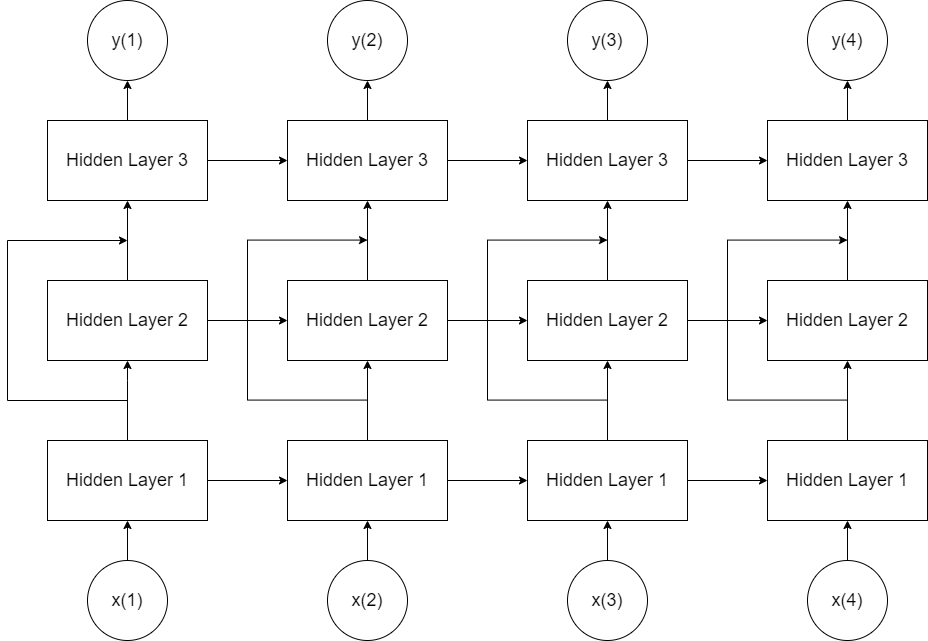
\includegraphics[width=250pt]{chapters/part-3/figures/rnn_general.png}
	\caption{An example of RNN.} \label{ch:rnn:fig:rnn_general}
\end{figure}

RNN has some limitations. One of the major problem is that it is difficult to train an RNN even for the basic standard feedforward networks. The optimization of RNN is NP-complete. It is especially difficult for RNN to learn long-range dependencies due to the vanishing and exploding gradients problem that could occur when backpropagating errors across many timestamps (long sequence) \cite{lipton2015critical}. This is one of the main challenges why RNN has difficulties building on long-range dependencies. The vanishing and exploding gradient problems are caused by the structure of the system as well as the backpropagation-based training methods.

Different approaches have been proposed to prevent vanishing and exploding gradient problems. Famous ones among these approaches include strategical weight initialization, long short term memory (LSTM), gated recurrent units (GRUs), skip connections, and more. Many of these approaches try to reduce the effect of vanishing and exploding gradient problems by carefully design the ANN structures. For example, both LSTM and GRUs introduce ``memory cells'' with built-in ``gates'' that balance and control the flow of information from previous cells versus current inputs. The cells are used to replace the traditional perceptron nodes. These approaches have made the training of RNN a feasible problem. LSTM and GRUs are almost certainly used in modern RNNs.

Bidirectional RNN (BRNN) is proposed at about the same time with LSTM. It allows information to travel not only from previous hidden layers to future layers, but also from future hidden layers to previous layers. LSTM and BRNN can be used together to boost the RNN performance. Notice that BRNN cannot run continuously as it requires fixed endpoints in both the future and the past. It is useful for prediction over a sequence of fixed length, such as part-of-speech tagging in natural language processing.

Another problem that people have found during the training of RNN is local optima. However, recent studies have shown that local optima is not as serious issue as we might thought when the network is large, since many critical points are actually saddle points rather than local minima.

Successful implementations of the above RNN structures include natural language translation such as \cite{sutskever2014sequence} where an encoder-decoder structure is used, each is an LSTM. Another example is image captioning, where the AI tries to explain what is in an image using texts. A solution to this is to use CNN to encode the image, and use LSTM to decode to generate texts. Following similar ideas is hand-writing recognition. 